\documentclass{article}
\usepackage{amsmath}
\usepackage{amsfonts}
\usepackage{amssymb}
\usepackage{graphicx}
\usepackage{listings}
\usepackage{verbatim}
\usepackage{wasysym}
%-------------------------------------------

\begin{document}

\title{Plug-in interface for Svarog\\ Tutorial}
\author{Marcin Szumski}
\maketitle

\tableofcontents

\section{Introduction}

Plug-in interface was created to allow the development of Svarog without the necessity to change its code.
In the long term it will increase the modularity of the project, as the code of the newly created plug-ins will
be independent from most of the Svarogs' code.
It should also result in a better stability, because it will be easier to locate in which plug-in the error occurs and simply switch the plug-in off.

There will be also a change from the user point of view, as he will be able to decide which extensions (from the set of plug-ins that may even exclude one another) he would like to use.

This tutorial is written with a lot of details, which for some developers may seem unnecessary or even foolish.
It is done on purpose, to make the creation of plug-ins possible also to non-advanced developers or simply those who don't know Java and Eclipse very well.
Moreover in this tutorial it is assumed that the plug-in is created in the Eclipse IDE.
Although anyone, who got accustomed to a different IDE and would like to use it shouldn't have a problem.

Below is a short schema, which operations the developer should perform to create a plug-in:
\begin{enumerate}
	\item create a new Java Project (section \ref{project}),
	\item add libraries to the build path (section \ref{libraries}),
	\item create a package and a starting class (section \ref{starting-class}),
	\item implement function \verb=register(SvarogAccess)= (section \ref{register}),
	\item write the functionality of the plug-in,
	\item export the project as a \verb=jar= file (section \ref{jar-export}),
	\item create an XML description (section \ref{XML-description}),
	\item put both files in the plug-in directory (section \ref{move}).
\end{enumerate}

\section{Creation of the project}
\label{project}
Go to: \verb=File -> New -> Project...=\\
Select: \verb=Java -> Java Project= and press \verb=Next >= \\
Type some custom \verb=Project name= (in our example it is \verb=ExamplePlugin=) \\
Press \verb=Finish=

\section{Adding libraries}
\label{libraries}
Next step is to add libraries to the build path:
\begin{itemize}
	\item Svarog snapshot (\verb=svarog-\{version\}.jar=) -
		the necessary library, which contains the Svarog classes (e.g. plug-in interface).
		Can be found in the directory \verb=svarog/target=.
	\item Apache log4j (\verb=log4j.jar=) - add this library if you want to use logging framework
		consistent with the one used in Svarog.
		This library can be found in the directory
		\small
		\begin{verbatim}svarog/target/svarog-\{version\}-full/svarog-\{version\}/lib\end{verbatim}
		\normalsize
	\item Spring Context (\verb=spring-context.jar=) - add this library if you want to use classes
		that inherit from \verb=MessageSourceAccessor= (e.g. \verb=Tag=, \verb=TagStyle=).
		This library can be found in the directory
		\small
		\begin{verbatim}svarog/target/svarog-\{version\}-full/svarog-\{version\}/lib\end{verbatim}
		\normalsize
\end{itemize}

In order to add libraries you need to:
\begin{itemize}
	\item copy selected libraries to the project directory,
	\item open \verb=Package Explorer=,
	\item right click on the project folder,
	\item select \verb=Build Path -> Configure Build Path...=,
	\item open tab \verb=Libraries=,
	\item click \verb=Add JARs...=
	\item expand project folder, select copied libraries and press \verb=OK=,
	\item again press \verb=OK=. 
\end{itemize}

\section{Creation of the starting class}
\label{starting-class}
In this section we are going to add a starting class that implements the interface
\begin{verbatim}org.signalml.plugin.export.Plugin \end{verbatim}
At the beginning let's create the package:
\begin{itemize}
	\item right click on \verb=src=, select \verb=New -> Package=,
	\item set the \verb=Name= to \verb=org.signalml.plugin.yourpluginname=\\
		(replace \verb=yourpluginname= with the name of your plug-in),
	\item press \verb=Finish=.
\end{itemize}
To the package add your starting class:
\begin{itemize}
	\item right click on the created package, select \verb=New -> Class=
	\item set the \verb=Name=,
	\item click \verb=Add..= to add an interface,
	\item type \verb=Plugin= and click \verb=OK=,
	\item press \verb=Finish=.
\end{itemize}

\section{\textit{register(SvarogAccess)} implementation}
\label{register}

\verb=Plugin#register(SvarogAccess)= is the only method that has to be implemented.
This method is called just after your plug-in is loaded and without it your plug-in won't
be able to communicate with Svarog (as only to this method the \verb=SvargoAccess= instance is passed).
Here should be :
\begin{itemize}
	\item added GUI elements (as adding them later won't be possible) (section \ref{gui}),
	\item registered listening on changes (section \ref{listeners}),
	\item performed all other operations that initialize the plug-in.
\end{itemize}

\section{Exporting project to jar file}
\label{jar-export}

When your plug-in is already created you have to export it to the \verb=jar= file.
To do it:
\begin{itemize}
	\item Open \verb=Package Explorer= and right click on the project folder.
	\item Click \verb=Export=.
	\item Select \verb=Java -> JAR file= and click \verb=Next=.
	\item Make sure your plug-in is selected, choose the export destination and press \verb=Finish=.
\end{itemize}

Note that Eclipse sometimes hangs during the export.
The best way to deal with it is to restart it.

\section{Creation of an XML file}
\label{XML-description}
Now it is the time to create an XML file, which describes the plug-in.
This file should contain some basic information about the plug-in.
Perhaps the easiest way to understand it is studying an example (figure [\ref{xml_listing}]).
\begin{figure}
\small
\label{xml_listing}
\begin{lstlisting}[frame=tblr]
<plugin>
  <name>
    Example plugin
  </name>
  <version>
    0.1
  </version>
  <jar-file>
  	ExamplePlugin.jar
  </jar-file>
  <starting-class>
    org.signalml.plugin.exampleplugin.ExamplePlugin
  </starting-class>
  <dependencies>
    <dependency>
      <name>
        Svarog API
      </name>
      <version>
        0.5
      </version>
    </dependency>
  </dependencies>
</plugin>
\end{lstlisting}
\caption{ExamplePlugin.xml}
\end{figure}

And here is the description of functions of xml tags:
\begin{itemize}
  \item \verb=<name>= - the \textbf{unique} name of the plug-in.
  \item \verb=<version>= - the version of the plug-in in the form of non-negative integers separated by dots.
  	The significance of the numbers is in the decreasing order (i.e. $2.1 > 1.9$).
  \item \verb=<jar-file>= - the name of the \verb=jar =file with the plug-in.
  	This jar file must be located in the same directory as the description (XML file).
  \item \verb=<starting-class>= - the fully-qualified name of the class that implements \verb=org.signalml.plugin.export.Plugin=
  	interface. The method register of this class will be called to load the plug-in.
  \item \verb=<export-package>= - the full name of the package that this plug-in wants to share with another plug-ins.
  	This field of the XML file is not used by Svarog and serves only as an information for developers of other
  	plug-ins (so that they can use some functions of this plug-in).
  \item \verb=<dependencies>= - the parent node for all dependencies (see next point).
  \item \verb=<dependency>= - describes the single dependency of this plug-in (another plug-in (or Svarog) that is required by this plug-in;
  	if at least one dependency is not satisfied, this plug-in won't be loaded).
  	
  	Each dependency contains two parameters of the plug-in (or Svarog) on which this plug-in depends:
  	\begin{itemize}
			\item \verb=<name>= - the name. Equal to the specified in the description of the plug-in.
			\item \verb=<version>= - the minimum version. The current version of the plug-in must be greater or equal to the specified here.
		\end{itemize}
		There is one special dependency that can be added - the dependency on Svarog Plugin API:
		\begin{itemize}
			\item \verb=<name>= - \verb=Svarog API=
			\item \verb=<version>= - the version of Svarog Plugin API - currently 0.5
		\end{itemize}
\end{itemize}

\section{Moving plug-in to plug-in directory}
\label{move}

Copy both exported the \verb=jar= file and the created description to the plug-in directory.
The default plug-in directory is located within your Svarog profile directory.
Now you can start Svarog and you should see your plug-in on the list \smiley

\section{Description of the elements of plug-in interface}

Below you will find the short description of functions provided in the plug-in interface.
Note that this is only a short introduction and if you want to learn something more you have to read JavaDoc \smiley.

Before we proceed to the description please read this two general remarks:
\begin{itemize}
	\item when you want to perform operations that require intensive computations use \verb=SwingWorker=\footnote{http://download.oracle.com/javase/6/docs/api/javax/swing/SwingWorker.html}.
		This class allows you to transfer computations outside \textit{Event Dispatch Thread}, so that you won't hang the entire GUI.
	\item with the plug-in interface are shipped some classes that are not necessary, but you may find them useful: \verb=AbstractDocument=, \verb=AbstractSignalTool=, \verb=SignalSelection=,
		\verb=SignalSelectionType=, \verb=Tag=, \verb=TagStyle=, \verb=AbstractDialog=, \verb=AbstractPopuDialog=, \verb=AbstractTreeModel=.
		For their description see JavaDoc.
\end{itemize}

\subsection{GUI elements}
\label{gui}
There are four types of GUI elements you can add:
\begin{enumerate}
	\item buttons - must implement interface \verb=javax.swing.Action=.
	To add them just call method \verb=addButtonTo*(Action)=.
	\item sub-menus - must be of type \verb=javax.swing.JMenu=.
	They can not contain sub-menus as the actions from them are copied to create menus
	e.g. for different signal plots.
	To add them just call method \verb=addSubmenuTo*(JMenu)=.
	\item signal tool - it is a mouse event processor associated with a single SignalView instance.
	To implement it you have to know a little more how Svarog works.
	The easiest way to create it is to extend \verb=AbstractSignalTool=, but if you do it you have to
	override method \verb=createCopy()= (and of course not throw \verb=UnsupportedOperationException=).
	
	For more information how the Signal Tools work, see some of the classes (\verb=RulerSignalTool=, \verb=SignalFFTTool=,
	\verb=Tag*SignalTool=, \verb=Select*SignalTool=).\\
	Adding a signal tool is done by calling the function \\
	\verb=addSignalTool(SignalTool, Icon, String, MouseListener)=,\\
	which adds to every SignalView, a button created from the provided elements and a COPY of provided signal tool.
	\item tabs - tabs can be added to 3 panes:
	\begin{itemize}
		\item main (center) pane - have to have type \verb=DocumentView=. Should be also associated with some
			\verb=Document= (which can be obtained from the view by method \verb=getDocument()=).
			These tabs are added by calling a function:
			\begin{verbatim}
				addMainTab(DocumentView tab, String title, Icon icon,
				             String tip)
			\end{verbatim}
		\item tree (left) pane - have to have type \verb=ViewerTreePane=, and therefore a \verb=JTree= associated with
			them.
			Can be added by calling:
			\begin{verbatim}
			addTreeTab(ViewerTreePane treePane, String title,
			                  Icon icon, String tip)
			\end{verbatim}
		\item property (bottom) pane - they only have to have type \verb=JPanel=, and there is no restrictions about
			them.
			Can be added by calling:
			\begin{verbatim}addPropertyTab(JPanel panel)\end{verbatim}
	\end{itemize}
\end{enumerate}
The addition of first 3 (buttons, sub-menus and signal tools) may be performed only during the initialization phase,
i.e. only in the function \verb=register(SvarogAccess)=.
Tabs can be added (and removed) at any time during the runtime of Svarog.



\subsection{Listening}
\label{listeners}
Listening for changes in Svarog is pretty simple, as it requires only to create a class, that implements a given listener
and to add this listener with methods from \verb=SvarogAccessChangeSupport=.

When the change, for which the added listener is listening occurs, the appropriate method in this listener is called
(e.g. if the \verb=Tag= is added the method \verb=SvarogTagListener#tagAdded= is called).
To this method is passed an event, which contains the objects that have changed.

Below are the possible types of listeners:
\begin{itemize}
	\item SvarogCloseListener - waits for the information that Svarog is closing
	\item SvarogCodecListener - waits for the information that the codec was added or removed.
		The event for the methods in this listener contains the format name of the added or removed codec.
	\item SvarogDocumentListener - waits for the information that the document was added/removed form Svarog,
		the active document has changed or the \verb=DocumentView= for the document changed.
		The events contain:
		\begin{itemize}
			\item for fist two methods (addition and removal) - only the added/removed document,
			\item for the third method (change of a view for a document) - the document and the old value of the changed view
				(as the new value can be obtained from document).
			\item for the fourth method (change of the active \verb=Document=) - old and new value of the active document.
		\end{itemize}
	\item SvarogTagDocumentListener - waits for the information that the active \verb=TagDocument= has changed.
		The event for the method in this listener contains the old and the new value of the active tag document.
	\item SvarogTagStyleListener - waits for the information that the \verb=TagStyle= was added, removed or changed.
		The event for the methods in this listener contains the changed tag style.
		
		This listener can be added to listen for all tag style changes or to listen for changes associated with the given
		tag or signal document.
	\item SvarogTagListener - waits for the information that the \verb=Tag= was added, removed or changed.
		The event for the methods in this listener contains the changed tag and the document in which the tag is located.
		
		This listener can be added only to listen for changes associated with the given	tag or signal document.
	\item SvarogTagListenerWithAcitve - it is the extension of \verb=SvarogTagListener=. Waits also for the change of an
		active tag.
		The event for the method associated with the change of the active tag contains the old and the new value of the active tag.
\end{itemize}

\subsection{Documents, samples and tags}
\label{signal}

\verb=SvarogAccessSignal= is an interface which allows to get from and add to Svarog some logical objects, namely:
\begin{itemize}
	\item Get samples from the signal - samples are available:
		\begin{itemize}
			\item either for the active signal or for the signal from the given document,
			\item either from a single channel or from all channels in the signal,
			\item either processed (after the montage and filtering) or raw (unprocessed).
		\end{itemize}
	\item Get tags - available are:
		\begin{itemize}
			\item tags from active or specified tag document
			\item tags from all tag documents dependent from the active or selected signal,
			\item tags from all tag documents
			\item the active tag
		\end{itemize}
	\item Add tags to the active or specified document.
	\item Open:
	\begin{itemize}
		\item a book or a signal file and add it as a tab,
		\item a file with codec and register a new codec,
		\item a file with tags and add it to the active or specified signal.
	\end{itemize}
	\item Get active elements:
		\begin{itemize}
			\item \verb=Document= - the document that is associated with the main tab,
			\item \verb=TagDocument= - the selected document with tags for the active signal,
			\item the tag,
			\item the selection of the part of the signal.
		\end{itemize}
\end{itemize}


\section{Plug-in options (in Svarog GUI)}

The plug-in options in Svarog GUI allow to: 
\begin{itemize}
	\item specify directories in which plug-ins are located,
	\item select which plug-ins should be active,
	\item check which plug-ins were not loaded because of an error,
	\item check which plug-ins have unsatisfied dependencies and see the list of these missing dependencies.
\end{itemize}
All accepted changes will take place after the restart of Svarog.

To show these options you need to go to \verb=Tools -> Plugins options=.
Dialog shown in figure \ref{plugin_options} should appear.

\begin{figure}
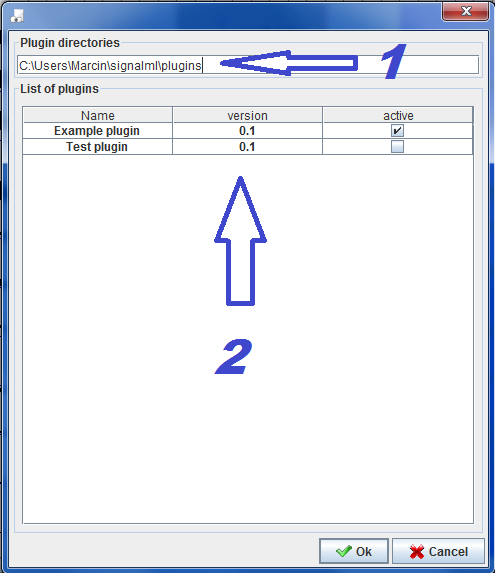
\includegraphics[width=0.8\textwidth]{plugin_options.png}
\caption{The dialog that allows to manage plug-ins.
In the text field in the panel $\mathbf{1}$ are paths to the directories in which the plug-ins are stored separated by semicolons.\newline
In the table $\mathbf{2}$ in every row one plug-in is displayed.
Third column of this table is editable, which allows user to select which plug-ins should be active.
}
\label{plugin_options}
\end{figure}

\begin{figure}
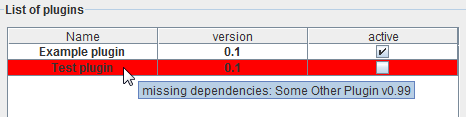
\includegraphics[width=0.8\textwidth]{missing_dependencies.png}
\caption{
If the plug-in is not loaded due to an error or missing dependency, the row with this plug-in is marked red and can't be edited.
Also if it is a missing dependency the tool-tip for this row, which enlists the missing dependencies, is set.\newline
Here: plug-in TestPlugin has a missing dependency - \textit{Some Other Plugin}, which should have version at least $0.99$.
}
\label{missing_dependencies}
\end{figure}

\end{document}
